\documentclass[12pt]{article}
\usepackage{amsmath}
\usepackage[pdftex]{graphicx}
\usepackage{natbib}
\usepackage[margin=1in]{geometry}
\usepackage{textcomp}
\usepackage{lineno}

%% for citing stuff in the supp
\usepackage{xr}
\externaldocument{dimensions_geb_supp}

%% make lists more compact
\usepackage{enumitem}
\setitemize{noitemsep,topsep=0pt,parsep=0pt,partopsep=0pt}
\setenumerate{noitemsep,topsep=0pt,parsep=0pt,partopsep=0pt}

\title{\vspace{-1em}Community assembly on isolated islands:
  Macroecology meets evolution}

\author{}

\date{}

%%%%%%%%%%%%%%%%% END OF PREAMBLE %%%%%%%%%%%%%%%%

\begin{document}
\baselineskip24pt
\maketitle 

\vspace{-4em}

A. J. Rominger$^{1*}$,
K. R. Goodman$^{1*}$, 
J. Y. Lim$^{2*}$, 
F. S. Valdovinos$^{3*}$, 
E. Armstrong$^{1, 4}$,
L. Becking$^1$,
G. M Bennett$^5$,
M. S. Brewer$^1$, 
D. D. Cotoras$^2$, 
C. P. Ewing$^4$, 
J. Harte$^1$,
N. Martinez$^3$,
P. O'Grady$^1$,
D. Percy$^6$,
D. Price$^4$,
G. K. Roderick$^1$,
K. L. Shaw$^7$,
D. S. Gruner$^{8\#}$,
R. G. Gillespie$^{1\#}$

\begin{enumerate}
\item Environmental Science, Policy, and Management, University of
  California, Berkeley, California 94720-3114
\item Integrative Biology, University of California, Berkeley,
  California 94720-3140
\item Pacific Ecoinformatics and Computational Ecology Lab, Berkeley,
  California 94703
\item Biology, University of Hawaii, Hilo, Hawaii, 96720-4091
\item Integrative Biology, University of Texas, Austin, Texas 78712
\item Entomology, The Natural History Museum, London, UK SW7 5BD
\item Neurobiology and Behavior, Cornell, Ithaca, New York 14853-7601
\item Department of Entomology, University of Maryland, College Park,
  Maryland 20742-4454
\item[*] Contributed equally; \# co-senior authors; 
\item[] corresponding author: R. G. Gillespie, gillespie@berkeley.edu.
\end{enumerate}


\vspace{2em}

\noindent
Keywords: networks, maximum entropy, arthropods, population genetics,
chronosequence, Hawaii

\noindent
Running title: Community assembly on isolated islands

\noindent
Number of words in the abstract: 330

\noindent
Number of words in main body of the paper: 5370

\noindent
Number of references: 66


\clearpage

\begin{linenumbers}

\section*{Abstract}

\paragraph{Aim}
Understanding how ecological and evolutionary processes
synergistically determine biodiversity patterns remains a central goal
in biology. In highly isolated archipelagoes such as the Hawaiian
Islands, beyond the reach of frequent colonization, rapid {\it in
  situ} diversification has the potential to keep pace with ecological
dynamics such as biotic filtering and demography in structuring local
biodiversity. Using ecological theory as a conceptual guide and data
from multiple arthropod lineages across the Hawaiian model system, we
explore how complex communities emerge from the interplay of
ecological (population dynamics, dispersal, trophic interactions) and
evolutionary (genetic structuring, adaptation, speciation, extinction)
processes.

\paragraph{Location}
The Hawaiian Islands ($19.5\textdegree$N, $155.5\textdegree$W).

\paragraph{Methods}
To infer processes involved in early diversification we synthesize
data on genetic structure of select arthropod species across Hawaiian
landscapes of known age. Across the range of geological ages of the
current high islands ($< 1$ my to 5 my) we also develop and analyze a
plant-herbivore bipartite network. We compare the structure of these
networks, measured by nestedness, modularity and the degree
distributions, with theoretical predictions derived from the principle
of maximum information entropy.

\paragraph{Results}
Based on the time perspective provided by the island chronosequence
and genetic information, we demonstrate that species in lower trophic
levels develop local divergence more quickly than species of higher
trophic levels. Higher trophic levels also show endemism, though it
evolves more slowly and over larger areas. Moreover, in analyzing
plant-herbivore networks across an increasing substrate age gradient
we find trends of higher specialization and increasing deviation from
the statistical steady state expected from theoretical predictions of
food web structure.

\paragraph{Main conclusions}
We show how ecological theory can leverage natural experiments on
oceanic islands of known chronologies to understand how the interplay
between evolutionary and ecological processes has shaped present-day
biodiversity. We advocate for combining perspectives gained from
coupled molecular and community-level data analyzed in the context of
ecological theory. Theory provides a lens through which to identify
interesting biological outliers. We further show the utility of applying
theory in a chronosequence context to better illuminate the interplay
of ecological mechanisms, speciation, extinction and adaptation in
driving contemporary biodiversity patterns.


\section*{Introduction}

Contemporary biodiversity is an unresolved product of speciation,
extinction and dispersal all conditioned by ecological interactions
with the biotic and abiotic environment.  Because these processes
occur on different temporal and spatial scales and may be interactive
with nonlinear feedbacks and lags among them, disentangling the
relative influence of local ecological mechanisms from evolutionary
and historical processes is challenging \citep{ricklefs2004}. The
integration of ecological and evolutionary theory has the potential to
reveal dynamics that generate biodiversity.

The evolutionary processes of speciation and extinction tend to be
viewed as regulating regional species pools, occurring in a manner
largely removed from local ecology \citep{hubbell2001,
  cavenderBares2009, wiens2011}. Ecological mechanisms tend to be
viewed as packing standing diversity into local communities through
competition, facilitation, and neutral ecological drift
\citep{hubbell2001, tilman2004, Bascompte2007, chase2011,
  borer2014}. Recent theoretical advances have further refined the
causes and consequences of ecological drift \citep{hubbell2001,
  rosindell2011, rosindell2012}, re-vitalized classical niche-based
mechanisms such as niche partitioning \citep{tilman2004, chesson2000},
competition and predation \citep{borer2014}, and put species
interactions in a network theoretic context \citep{williams2000,
  brose2006, berlow2009}. The combined advances of ecological theory,
with its broad predictive power, and insights into evolutionary
mechanisms based on inference from contemporary patterns of species,
genetic, or phylogenetic diversity \citep[e.g.,][]{kreft2007,
  jetz2012, wiens2004, wiens2011} have set the stage to address
longstanding questions of how evolutionary history can drive common
patterns in contemporary ecology \citep{ricklefs1987}. Here, we
propose an integrative framework to study evolutionary community
assembly. We then provide an initial test using arthropod lineages in
the model archipelago of the Hawaiian Islands using mostly published
data.  We estimate metrics of evolutionary and ecological dynamics
across communities that range in age from 500 yr to 5 myr: (1) The
timeline for the development of genetic discontinuity and the extent
to which taxa across communities differ in the rates that populations
change from panmixia to fully differentiated species. This is
contextualized with (2) macroecological metrics of community
structure, using predictions from statistical steady state and
ecological network theory to examine changes over the island
chronosequence.

\subsection*{Hotspot oceanic archipelagos as model systems}

Hotspot oceanic island systems are opportune model systems for
studying the interplay of local ecological mechanisms and
large--scale, historical, and evolutionary drivers of biodiversity
patterns. Such island systems are discrete in space and in time due to
their sequential formation as the tectonic plate moves over a volcanic
hotspot.  We hypothesize that the contributions of evolutionary and
ecological assembly will vary according to geological age of the
environment, taken as an indicator of the total time communities have
had to assemble and over which {\it in situ} diversification could
occur.  Age--structured, hot--spot island archipelagoes thus have the
potential to stratify the eco--evolutionary process of community
assembly.

For example, younger communities by necessity originate mostly from
initial immigration (from neighboring older volcanoes and islands or
from the mainland, depending on the level of isolation), and thus
should be dominated by ecological mechanisms operating on a source
pool whose evolution is removed from the local setting. Conversely,
older islands could allow observation of the combined interaction and
feedback of the diversification of the source pool and local
ecological dynamics.  The temporal stratification within such
archipelagoes hence provides an opportunity to disentangle these
interacting processes. Moreover, because dispersal, and hence
connectivity between sites, differs between taxa, the relative role of
evolutionary and ecological assembly will differ between taxa. While
many archipelagos around the world share these biotic and geologic
properties, the Hawaiian archipelago provides a particularly useful
system for study because its geological chronology \citep{price2002}
and patterns of biodiversity are well characterized
\citep{wagnerFunk}.


\subsection*{Development of genetic discontinuity}

Movement of individuals among localities connects the population
dynamics of those localities.  Even moderate levels of genetic
connectivity among geographically separated populations limits the
potential for local divergence \citep{wright1978, slatkin1987}.  Thus,
in the face of connectivity among populations, one predicts that the
structure of ecological communities will remain similar across space.
By contrast, when connectivity is low, not only are the ecologies of
populations in different localities free to vary, but genetic
divergence is also more likely.  For these reasons, the magnitude of
connectivity among population provides a measure of the relative
importance of ecological processes and evolutionary processes in
determining differences among ecological communities.  Here, by using
the chronosequence, we can apply this approach to sets of communities
from young to old and to taxa representing different trophic levels.


\subsection*{Macroecological metrics}

While we expect the mechanisms underlying the generation and
maintenance of biodiversity to change across chronological sequences,
studies to date have rarely moved beyond reporting basic patterns
\citep{gillespieBaldwin}. Theory provides a necessarily simplified
view of biodiversity and deviations from theory can reveal which more
biologically realistic mechanisms likely underlie observed
patterns. The Maximum Entropy Theory of Ecology
\citep[METE;][]{harte2011} provides a prediction for idealized
ecological communities in statistical steady state. Statistical steady
state describes the situation in which a system's behavior is governed
by a simple set of state variables and no further system-specific
mechanisms are required \citep{harte2011, harte2014}. Thus METE, while
in a sense neutral, makes fewer assumptions than neutral theory
\citep{hubbell2001}, allowing for the possibility that myriad
ecological mechanisms influence communities. However, METE assumes
that these mechanisms have no statistical effect on the macroscopic
biodiversity patterns of the system. Real world deviations from METE
can provide insights into the processes driving ecology away from this
statistical steady state and toward alternate system states
\citep{harte2011}. We expect that different aged communities along the
Hawaiian chronosequence will deviate differently from METE, because we
hypothesize the processes of speciation, extinction, adaptation and
colonization may themselves drive Hawaiian communities out of
statistical steady state.

METE can successfully predict various metrics of an ecological
community \citep{harte2011}, including network metrics that describe
trophic interactions between species \citep{williams2010,
  harte2011}. Ecological network theory incorporates evolutionary
concepts such as coevolution \citep{Bascompte2007, Donatti2011,
  Nuismer2013} and has clear ties with macroecological questions of
the distribution of abundance and body size across species
\citep{berlow2009, williams2010, harte2011}. The distribution of
linkages in ecological networks has been used to determine whether
plant-animal interaction networks assemble neutrally or through
deterministic processes \citep{Vazquez2005}. Analysis of other network
metrics such as modularity (the degree to which species interact in
semi-autonomous modules) and nestedness (the degree of asymmetry in
interaction between specialists and generalists) can further
illuminate underlying eco-evolutionary processes driving patterns of
species interactions \citep{Bascompte2007, Donatti2011, Nuismer2013}.

In this paper we integrate methods from population genetics to
theoretical ecology using the chronosequence of the Hawaiian
Archipelago to understand the nexus between ecological and
evolutionary forces community assembly. Moving rom young to old across
the chronosequence we evaluate (1) the rate and pattern of genetic
connectivity among populations of taxa from different trophic levels
as they diversify from populations to form new species; (2) the
processes underlying the structure of species interaction networks
given the backdrop of population divergence; and (3) the processes
involved in diversification as species form and accumulate and how
this dynamic drives deviations from statistical steady state. We use
data (mostly published) on population genetic structure and species
interactions as a proof of concept. With this framework, our goal is
to show how communities develop over ecological-evolutionary time, and
the dynamic feedbacks involved assembly.


\section*{Methods}

\subsection*{Hawaii as an eco-evolutionary study system}

The geological landscape of the Hawaiian Islands offers a matrix of
volcanic substrates mapped in fine detail by chronological age and
geochemical composition \citep{sherrod2007}. On Hawaii Island in
particular, independent gradients in elevation and precipitation
interact within a matrix of substrate ages ranging from contemporary
(active) to 500,000 years. Ongoing volcanic activity has created a
dynamic mosaic of habitats with transitory to long-lasting
fragmentation within landscapes. Isolation on scales of hundreds to
thousands of meters and hundreds to thousands of years can be
sufficient for genetic differentiation among some arthropod
populations among habitats \citep{goodman2012, eldon2013,
  bennett2013}, while insufficient to isolate others
\citep{vandergast2004}. On larger spatial and temporal scales,
distinct volcanoes and islands, with their semi-independent histories
of evolutionary community assembly from recent to ancient, comprise a
space-for-time geological chronosequence spanning from present day up
to 5 million years across Hawaii Island to Kauai.

To investigate how ecological patterns change in response to varied
evolutionary contexts we selected four focal sites across the
chronosequence of substrate and island ages (two on Hawaii Island, one
on Maui and one on Kauai). Focal sites were selected to have similar
forest composition (dominated by {\it Metrosideros polymorpha}:
Myrtaceae), elevation (1100-1400m), and climate (mean annual
precipitation 2000-3000 mm), while deliberately varying substrate
age. These forested montane sites are well-studied and primarily
composed of native plant and arthropod species .  The four sites span
the chronosequence from 0.0002–5 million years (Kilauea and Kohala
(Hawaii Island); Waikamoi (Maui), Kokee (Kauai); see
Fig. \ref{fig:map}).

\subsection*{Compilation and analysis of genetic data}

To evaluate the balance between region immigration and potential for
local ecological differentiation, we measured how molecular variation
is partitioned within species within locations of known substrate age
on Hawaii Island and Maui. We compiled published and new data sets for
a diversity of native Hawaiian arthropod groups that represent a
spectrum of trophic levels:
\begin{enumerate}
\item Herbivorous {\it Nesosydne} planthoppers \citep[COI and
  microsatellites;][GenBank accession numbers XXX-XXX]{goodman2012};
  {\it Trioza} psyllids (COI, cytB; GenBank accession numbers
  XXX-XXX); and fungivorous {\it Drosophila sproati}:
  \citep[COII;][]{eldon2013} that maintain tight host plant
  associations.
\item Detritivorous {\it Laupala} crickets
  \citep[AFLPs;][]{mendelson2004}; and
\item several predatory spiders species \citep[COI and
  allozymes;][]{roderick2012, croucher2012}
\end{enumerate}

In the case of previously unpublished molecular data, sequences for
{\it Nesosydne} planthoppers were generated following protocols
described in \citep{goodman2012} and sequences for {\it Trioza}
psyllids were generated following protocols described in
\cite{percy2003} with primers given in \cite{simon1994} and
\cite{timmermans2010}. Existing genetic data from across Hawaii Island
and Maui (including, but not limited to the focal sites), provide an
estimate of how arthropod populations have accumulated genetic
diversity and divergence within the dynamic landscape of the focal
sites.

We used analysis of molecular variance (AMOVA) to examine how genetic
variation is partitioned at two scales of population structure: among
sites within volcanoes and among volcanoes on both Hawaii Island and
Maui Nui. All analyses of allozyme and DNA sequence data were
performed in Arlequin v. 3.5 \citep{arlequin} using the AMOVA
procedure to compute $F_{ST}$, a measure of genetic variance, or,
where possible $Phi_{ST}$, an $F_{ST}$ analog that incorporates
genetic sequence information. The {\it Laupala} AFLP data were analyzed
using TFPGA v. 1.3 \citep{miller1997}, using the same hierarchical
approach as described above. To provide a temporal framework for the
population differentiation analysis we assembled divergence dating
information from the literature for as many of the taxa as possible
and additionally implemented a new divergence dating analysis for
{\it Tetragnatha} spiders (see supplementary information).

To explicitly evaluate the role of landscape age in allowing {\it in
  situ} genetic diversity and potential for divergence we analyzed how
within site $F_{ST}$ varies with the geologic age of volcanoes on
Hawaii Island and Maui Nui. For each volcano we calculated $F_{ST}$ or
$\Phi_{ST}$ \citep{arlequin} for each taxon between sites within
volcanoes.

\subsection*{Construction of plant-herbivore networks}

Bipartite networks describe the topology of ecological interactions
between two guilds of organisms (e.g. herbivores and their plant
hosts). Quantitative information on the relative importance of
interaction links can be incorporated into network analyses
\citep{Vazquez2009}; however, currently available data are restricted
to binary networks, those that describe only the potential for
interaction between any two species, but not the relative frequency of
that interaction to each species.

We compiled species lists of all endemic hemipteran herbivores for
each focal site from published species accounts (see supplement for
full list). Species accounts and other published sources were used to
determine the presence, probable presence, or probable absence of each
Hemiptera species at each of our four focal sites. A documented
presence was defined as a known specimen collected at the focal site;
a probable presence was defined as a species whose abiotic tolerances
and known geographic range (see supplement) overlap with a focal site
but no known specimen exists confirming its presence. Probable absence
was assumed when neither criteria for presence or probable presence
are met. Two sets of species lists for each focal site were compiled:
a conservative data set composed of only documented presence
occurrences and a less conservative data set that also included
probable presences.

Host plants for each hemipteran species were determined from published
species accounts. Data on host plant use at each specific site were
not available so we assumed that if a known host plant was present at
a site it would eventually be used. Host plant occurrence in the focal
sites was determined using distribution models for 1158 species of
Hawaiian plants \citep{price2012}. Each focal site was spatially
joined in a geographic information system with all coincident plant
distribution models that fell within its boundaries. Two sets of
resulting focal site-specific networks were constructed: one using the
conservative data set of hemipteran species presences and the other
using the less conservative data set.

\subsection*{Analysis of plant-herbivore networks}

We hypothesize that communities differentially depart from statistical
steady state along the continuum form those dominated by ecological
processes to those with potential complex evolutionary feedbacks We
used METE \citep{williams2010, harte2011} to compute the statistical
steady state for the hemipteran degree distribution (distribution of
the number of plant hosts to each hemipteran species). To evaluate how
well METE predicts the data we simulated METE-conforming communities
of the same number of species and links as observed. We then
calculated the log-likelihood of each simulated data set and compared
the resultant distribution of log-likelihoods under the hypothesis
that METE is true, to the observed log-likelihood. This comparison is
identical in approach to a z-score test using a Monte Carlo simulation
to estimate the sampling distribution of log-likelihoods. {\tt R}
scripts used for METE estimation and Monte Carlo methods are
available in the supplement.

To further investigate how {\it in situ} diversification leaves a
potentially unique signature on network structure we analyzed the
number of links assigned to each hemipteran species (the degree
distribution) separately for island endemics (those species found on
only one island and thus likely derived from in situ diversification)
versus island cosmopolitans (those species found on multiple
islands). To compare species' degree distributions between endemics
and cosmopolitans across sites of different ages we conducted a
generalized linear model with binomial error, treating site identity
as a categorical predictor. Binomial errors effectively account for
network size due to the bounded support of the binomial distribution.

To understand how other network properties change with ecosystem
substrate age, we calculated two widely used descriptive network
metrics across sites---nestedness, which describes the degree of
asymmetry of species interactions connecting specialists and
generalists \citep{Bascompte2003, Ulrich2009}, and modularity which
describes the degree to which interactions are concentrated within
subsets of species but not between subsets \citep{Newman2004,
  Olesen2007}.

We calculated nestedness using the NODF metric \citep{nodf} as
implemented in the {\tt R} package {\tt vegan} \citep{vegan} and
modularity using a variety of algorithms implemented in the {\tt R}
package {\tt igraph} \citep{igraph}. These metrics are not directly
comparable across networks of different size and connectance
\citep{Ulrich2009}, so for each metric in each network we calculate
z-scores using a null model that randomizes network structure while
maintaining certain aggregate network properties
\citep{Ulrich2009}. These z-scores are calculated as the difference
between the observed network metric minus the mean of the null model
divided by the null model standard deviation, or
($x_{obs}-\bar{x}_{sim})/sd_{sim}$). Because z-scores can be highly
sensitive to the choice of null model \citep{Ulrich2009} we
implemented both a probabilistic null model \citep{Bascompte2003} and
a null model that strictly constrains the degree distributions of
plants and herbivores \citep{Ulrich2009}. The probabilistic null using
the frequency of interactions as the probability that a randomized
link gets assigned to that cell in the interaction matrix
\citep{Bascompte2003}; thus the probabilistic null constrains row and
column sums in probability but not absolutely.

\section*{Results}

\subsection*{Population genetic inference of discontinuity among
  populations}

The analysis of molecular variance (AMOVA) revealed evidence of
significant population genetic structure from the smallest to the
largest spatial scales examined, all within a very recent
timeframe. For mitochondrial loci, the amount of statistically
significant molecular variation partitioned to among sites within
volcanoes ranged from 0.037–-0.92 and to the among volcanoes from
0-–0.30. Corresponding variation at multilocus nuclear loci
between-sites within volcanoes ranged from 0.21-–0.58 and among
volcanoes, 0.04–-0.34. Taxa in the lower trophic levels (herbivorous
sap-feeding Hemiptera: planthoppers and psyllids) had as much or more
molecular variation partitioned at the among-site, within volcano
level than the among volcano level, while the predatory spiders were
less structured at localities within volcanoes compared to between
(Table \ref{tab:fst}). The analysis of genetic population structure
across the chronosequence of localities revealed a similar
pattern. The herbivores show high genetic population structure among
localities on young volcanoes relative to between localities on older
volcanoes (Fig. \ref{fig:volcanoFst}). By contrast, predatory spiders
exhibited higher genetic population structure only on older volcanoes
(e.g. Maui).

The observed levels of genetic divergence have evolved rapidly. For
example, within species genetic divergence in planthoppers has evolved
in as little as 2,600 years \citep{goodman2012}. For species from
Hawaii Island for which phylogenetic data provide divergence times,
estimates of dates of species divergence range from 0.34–1.15 million
years, with additional within-species genetic divergence developed
subsequently (Table \ref{tab:fst}).

\subsection*{Evolving network structure}

The Hemiptera species degree distribution varied across the
chronosequence with both the youngest and oldest sites deviating most
from the statistical steady state maximum entropy predictions
(Fig. \ref{fig:degree}). In the middle aged site of Kohala, minor
deviations from maximum entropy are no different than expected by
chance indicating the Kohala Hemiptera assemblage matches the
predictions of maximum entropy.

The generalized linear model revealed that there are also significant
differences between the degree distributions of island endemics (those
species found on only one island) versus island cosmopolitans (those
species found on multiple islands; Fig. \ref{fig:degree}). Endemics
show significantly lower degree distributions overall (i.e., more
specialization) compared to more generalist cosmopolitan
species. Endemics become significantly more generalist on the middle
aged Maui site; however this pattern disappears when analyzing links
to plant genera instead of species. The slightly younger Kohala shows
increased generalization overall. When considering the degree
distribution defined by trophic links to plant genera instead of plant
species, the pattern of increased generalization holds for the Kohala
but endemics on Maui no long show a difference in their degree
distributions from other island endemics. This change in pattern
suggests that increased generality of Maui endemics may be driven by
increased intra-genus plant diversity on that island.

Network nestedness decreased with age while modularity increased
(Fig. \ref{fig:netMet}). This trend is found in networks constructed
from both more and less stringent geographic criteria (supplemental
Fig.  \ref{figSupp:netCons}). Choice of null model changed the
magnitude of modularity and the sign of nestedness z-scores; however,
the relative pattern of decreasing nestedness and increasing
modularity remained across the different null models used to
standardize network metrics (supplemental
Fig. \ref{figSupp:netMetComp}). The patterns are also robust to
sampling intensity, as demonstrated by a rarefaction analysis
(supplemental Fig. \ref{figSupp:rfy}).

\section*{Discussion}
By combining disparate data with a novel combination of analytical
approaches that incorporate population genetics, bipartite networks
and maximum entropy theory, our results present evidence for the
timeline over which evolution begins to keep pace with ecology in
determining the local diversity of communities. Taxa in the lower
trophic levels, as compared to higher trophic guilds, developed
genetic discontinuities more quickly along the chronosequence and at
much smaller spatial scales (Table \ref{tab:fst},
Fig. \ref{fig:volcanoFst}), allowing them the opportunity to diverge
ecologically. Network nestedness decreased while modularity increased
with age (Fig. \ref{fig:netMet}), indicating a possible shift from
assembly driven by {\it ex situ} immigration early on, to one based on
{\it in situ} co-diversification with host plants
\citep{Bascompte2007, Donatti2011}. This possibility is further
strengthened by the observation that single island endemics show more
specialization compared to more broadly distributed species
(Fig. \ref{fig:degree}). At intermediate modularity and nestedness,
the distributions of the number of links assigned to each hemipteran
species showed the least deviation from the METE prediction (Fig.
\ref{fig:degree}), suggesting that at the transition from primary
succession to evolutionary assembly, these plant-herbivore communities
reach statistical steady state. 

\subsection*{Development of genetic discontinuity at different trophic
  levels}

The analysis of available genetic data presented here indicates that
divergence is occurring within the islands at small spatial scales and
over short time periods (Table \ref{tab:fst},
Fig. \ref{fig:volcanoFst}). Furthermore, the scale of population
structure varies with trophic position, with the sap-feeding
herbivores in this study showing structure at smaller scales compared
to detritivorous crickets and predatory spiders (Table \ref{tab:fst},
Fig.  \ref{fig:volcanoFst}). Population structure within species
allows for populations to take independent evolutionary trajectories,
especially when aided by other evolutionary processes that may be
acting differentially across each species' range. A variety of factors
have been implicated in the genetic divergence of populations and
species in lineages described here, including combinations of genetic
drift associated with geographic isolation \citep{percy2003,
  gillespie2005, mendelson2005, ogrady2011, goodman2012}, adaptation
associated with ecological interactions of competition, predation, and
mutualism \citep{gillespie2004, blackledge2005, roderick2008}, and
sexual signaling \citep{mendelson2005, percy2006, magnacca2008,
  goodmanInRev}.

The sap-feeding Hemiptera group {\it Nesosydne} \citep{goodman2012}
provide evidence that some period of geographic isolation preceded
divergence of sexual signals \citep{goodmanInRev}. Shifts in plant
host use are also involved in the process of diversification in this
group \citep{roderick2008}. In a similar radiation of leafhoppers,
{\it Nesophrosyne} \citep{bennett2013}, host plant specialization was
implicated in driving species radiations up until approximately 1
million years ago, when plant niches were mostly exhausted on Maui;
following this period, speciation, largely on the Hawaii Island,
shifted to geographic mechanisms of diversification. Our network
analysis indicates that specialization and modularity begin to show
pronounced signals in network data on Maui (Figs. \ref{fig:netMet},
\ref{fig:degree}), in agreement with the {\it Nesophrosyne} results
and indicating that an approximate age of 1 million years may be
necessary for host plant specialization to become the dominant process
in the sequence of diversification. Other taxa at lower trophic
levels, such as the herbivorous {\it Trioza} psyllids, detritivorous
{\it Laupala} crickets and fungivorous {\it Drosophila}, show similar
signals of geographic isolation combined with ecological and sexual
processes driving genetic divergence and diversification across sites
as young as those on the Hawaii Island \citep{percy2003,percy2006,
  mendelson2005, magnacca2008, ogrady2011}. As a contrast, spiders,
which are predatory, only develop genetic discontinuities at larger
spatial and temporal scales.  Most important in the context of
community assembly is that endemic sap-feeding herbivores developed
structure quickly (on the order of less than 0.1 million years; Table
\ref{tab:fst}), with predatory spiders showing local endemicity more
slowly (Table \ref{tab:fst}).

\subsection*{Macroecological metrics: Network structure and steady
  state}

On the geologically youngest volcano, Kilauea, ecological assembly
should be the dominant process there. The results of network analysis
support this hypothesis with Kilauea showing substantial nestedness
and limited modularity (Fig. \ref{fig:netMet}). Nestedness is likely
to result if new species arriving by immigration have a high
probability to eat or be eaten by the generalist species already
present at the site \citep{Bascompte2003}. In this way we might expect
Kilauea to also conform to the statistical steady state predication of
maximum entropy. However, the observed deviations from maximum entropy
at Kilauea are largely driven by a surplus of singleton links (Fig.
\ref{fig:degree}). These in turn likely result from incomplete
assembly, and thus lower species richness, of the plant and herbivore
biotas. Future research should focus on the observation from genetic
analysis that indicates discontinuities can arise within species on
short timescales that, in some taxa, include the greater landscape of
Kilauea (Table \ref{tab:fst}).  Conversely, Kohala shows a
statistically significant agreement with maximum entropy perhaps
because the Kohala site, at intermediate age (150 ky), has experienced
complete ecological succession but is still too young to be driven
away from statistical steady state by specialization and rapid in situ
diversification driven by host plant preference

The older Maui and Kauai sites show strong deviations from
expectations of maximum entropy theory (Fig. \ref{fig:netMet}), which
is consistent with our hypothesis that the influence of evolutionary
assembly on these biotas drives them away from statistical steady
state. The application of maximum entropy to ecology does not
currently take into account evolution \citep{harte2011}. Indeed the
use of maximum entropy in ecology is inspired by its application to
physical systems whose change through time is simple and lacks the
evolutionary memory of biological systems, potentially a far cry from
the complex change through time produced by speciation, extinction and
adaption to novel ecosystems \citep{eldredge1989}. Maui
and Kauai show strong evidence of evolutionary assembly driven by
specialization and diversification on host plants, particularly
demonstrated by decreased nestedness and increased modularity
(Fig. \ref{fig:netMet}). Modularity is known to result from
coevolution selectively driving the traits of interacting species
towards convergence \citep{Donatti2011, Nuismer2013}.

The analysis of island endemic and cosmopolitan (archipelago-wide)
Hemiptera species sheds further light on the evolution of the networks
they form. Endemics are always more specialized than cosmopolitans,
further supporting the hypothesis that in situ diversification and
evolutionary assembly favor coevolution. At the Kohala site , which
showed the best fit to maximum entropy theory, endemic and
cosmopolitan species alike show increased generalization (i.e. higher
degree; Fig \ref{fig:degree}), while at the youngest site Kilauea,
specialist endemics are limited by low plant diversity and thus show
more apparent specialization (Fig \ref{fig:degree}). Conversely at the
oldest site on Kauai, where plant diversity is not limiting
\citep{kitayama1995}, endemics again show decreased degree and thus
genuine specialization (Fig. \ref{fig:degree}). On Maui, endemics show
statistically significant increases in apparent generalization but
this pattern disappears when analyzing the data at the resolution of
plant genera, thus suggesting that Hemiptera species endemic to Maui
are no more generalized on plant genera but instead may benefit from
the diversification of plant species within genera on Maui.

\subsection*{Future Research}

The analyses presented here indicate strong patterns of a dynamic
assembly process leading to contrasting hypotheses concerning the
relative importance of ecological and evolutionary depending on the
evolutionary age of the community under observation. In future work we
will tackle these hypotheses using detailed quantitative ecological
and genomic data collected from across the Hawaiian archipelago.
\begin{enumerate}
\item In younger communities we hypothesize that
  \begin{enumerate}
  \item during periods of ecological assembly, communities strongly
    influenced by immigration will resemble random samples from
    regional source pools and thus metrics describing these
    communities will largely match expectations of statistical steady
    state after primary succession has completed;
  \item the exception will be communities still undergoing primary
    succession, which will change rapidly through time
    and represent non--random samples of source pools;
  \item we also predict that these communities will exhibit a nested
    network structure, assuming new species will eat or be eaten by
    the generalist species \citep{Bascompte2003} already present in
    the community.
  \end{enumerate}
\item Following the same logic, in older communities we hypothesize
  that
  \begin{enumerate}
  \item during periods of evolutionary assembly, if processes such as
    niche exploration, adaptation and speciation happen fast enough to
    keep pace with immigration, the resultant communities could be
    driven into alternate evolutionary states that fail to meet the
    predictions of purely statistical theories that do not account for
    evolutionary dynamics \citep{harte2011};
  \item networks in such communities should exhibit higher levels of
    specialization and modularity \citep{Bascompte2007, Donatti2011,
      Nuismer2013}.
  \end{enumerate}
\item Systems undergoing rapid ecological and evolutionary change are
  generally expected to deviate most from statistical steady state;
  thus we expected populations in such communities to show genetic
  signatures of rapid change, from bottlenecks or population expansion
  to selection.
\end{enumerate}

\subsubsection*{Evolutionary data: Diversification within species}

The current study demonstrates that taxa of different trophic guilds
differ in the scale at which differentiation occurs, and highlights
the importance of fragmentation of the landscape in facilitating
differentiation. For some taxa fragmentation clearly allows genetic
separation. For others, in particular those that are more connected,
the fragmentation can provide a way of enhancing adaptive
differentiation \citep{gillespie2014}. Future work is aimed at
gathering genomic SNP data for focal taxa within this system that
represent different trophic levels. We will use it to understand
taxonomic differences in the rate of differentiation, to assess the
roles of genetic fusion and fission, and to detail the relative rates
of speciation and extinction across the island chronosequence.

For lineages characterized by extensive ecological diversification,
recent work has highlighted the potential role of multiple
colonizations and admixture in enhancing variability: while a break in
gene flow is necessary for adaptive differentiation, hybridization and
genetic admixture are key in the generation of adaptive variation and
functional novelty \citep{seehausen2004, rius2014}. Numerous studies
demonstrate that the negative effects of genetic founder effects may
be offset if different colonization events result in multiple
genotypes within the introduced population \citep[see][and citations
therein]{rius2014}. This highlights the potential role of admixture
among successively introduced populations in providing the genetic
variation to allow adaptive evolution over surprisingly short time
scales.


\subsubsection*{Ecological data: Assembly of species into communities}

Our results show that the island chronosequence can reveal important
insights into the process of community assembly, namely that
ecological processes dominate in younger environments, with
evolutionary processes becoming more important later. However, in
order to understand the nature of the assembly process and the dynamic
nature of the feedbacks involved, future work is focusing on
conducting broad sampling of all macroscopic arthropod taxa at a
number of sites across the age gradient, thus allowing assessment of
changes in overall species composition and diversity across all
players in the time-calibrated landscape \citep[{\it
  sensu}][]{gruner2007}.

Such data will also allow us to test how entire arthropod communities
of different aged substrates deviate from statistical steady state as
predicted by METE \citep{harte2011}. For example, predators, whose
assemblages are likely more dominated by immigration and ecological
assembly (Fig. \ref{fig:volcanoFst}) are hypothesized to never show
strong deviations from METE predictions whereas herbivores are
hypothesized to show increasing deviation with age and potentially at
the youngest sites as well in agreement with the network results of
this paper (Fig. \ref{fig:degree}).

The current study provides a framework for the use of chronologically
arranged oceanic island systems to examine the interplay between
evolutionary and ecological processes in shaping biodiversity. We
analyze preliminary molecular and community--level data together in
the context of ecological theory to demonstrate how this approach can
provide insights into how communities develop over
ecological--evolutionary time, and the dynamic feedbacks involved in
assembly.


\section*{Acknowledgement}
We are indebted to many scientists and land managers in Hawaii that
have provided access to the lands: Pat Bily (The Nature Conservancy of
Hawaii), Melissa Dean, Christian Giardina, and Tabetha Block (Hawaii
Experimental Tropical Forests), Betsy Gagne (Natural Area Reserve
System), Lisa Hadway and Joey Mello (Department of Forestry and
Wildlife Hilo), Cynthia King and Charmian Dang (Department of Land and
Natural Resources), and Rhonda Loh (Hawaii Volcanoes National
Park). We thank Robert Ricklefs, Lauren Ponisio and Anna Hiller for
thoughtful commentary. We are very grateful to Guida Santos, Richard
Field and Robert Ricklefs for inviting us to contribute to this
special issue. The research was supported by the National Science
Foundation DEB 1241253.


\bibliographystyle{geb}
\bibliography{dimensions_geb}

\clearpage

\section*{Biosketch}

The authors are part of a large team involved in understanding how
biodiversity and complex ecosystems emerge from ecological and
evolutionary processes. The project, funded by the National Science
Foundation's ``Dimensions in Biodiversity'', focuses on the geological
chronosequence provided by the Hawaiian Islands. Each of the
co-authors are involved in the effort, although Rominger, working
closely with Goodman, Lim, and Valdavinos, played the key role in
tying the elements together for the current
manuscript. Macroecological tools that have been employed for the
study include those developed by Harte and Martinez. From the more
empirical side, Gruner has long standing projects in the Hawaiian
Islands on the ecological underpinnings of community
diversity. Rominger, Lim and Fernandez bring a macroecological
perspective to the project. From the evolutionary perspective, Shaw's
research focuses on {\it Laupala} crickets; Ewing on nitidulid
beetles, Goodman Bennet and Roderick on Hawaiian planthoppers; Percy
on endemic psyllids; O'Grady and Price on Hawaiian {\it Drosophila};
and Cotoras with Gillespie on spiders.

\section*{Tables}

\begin{table}[!htb]
  \centering
  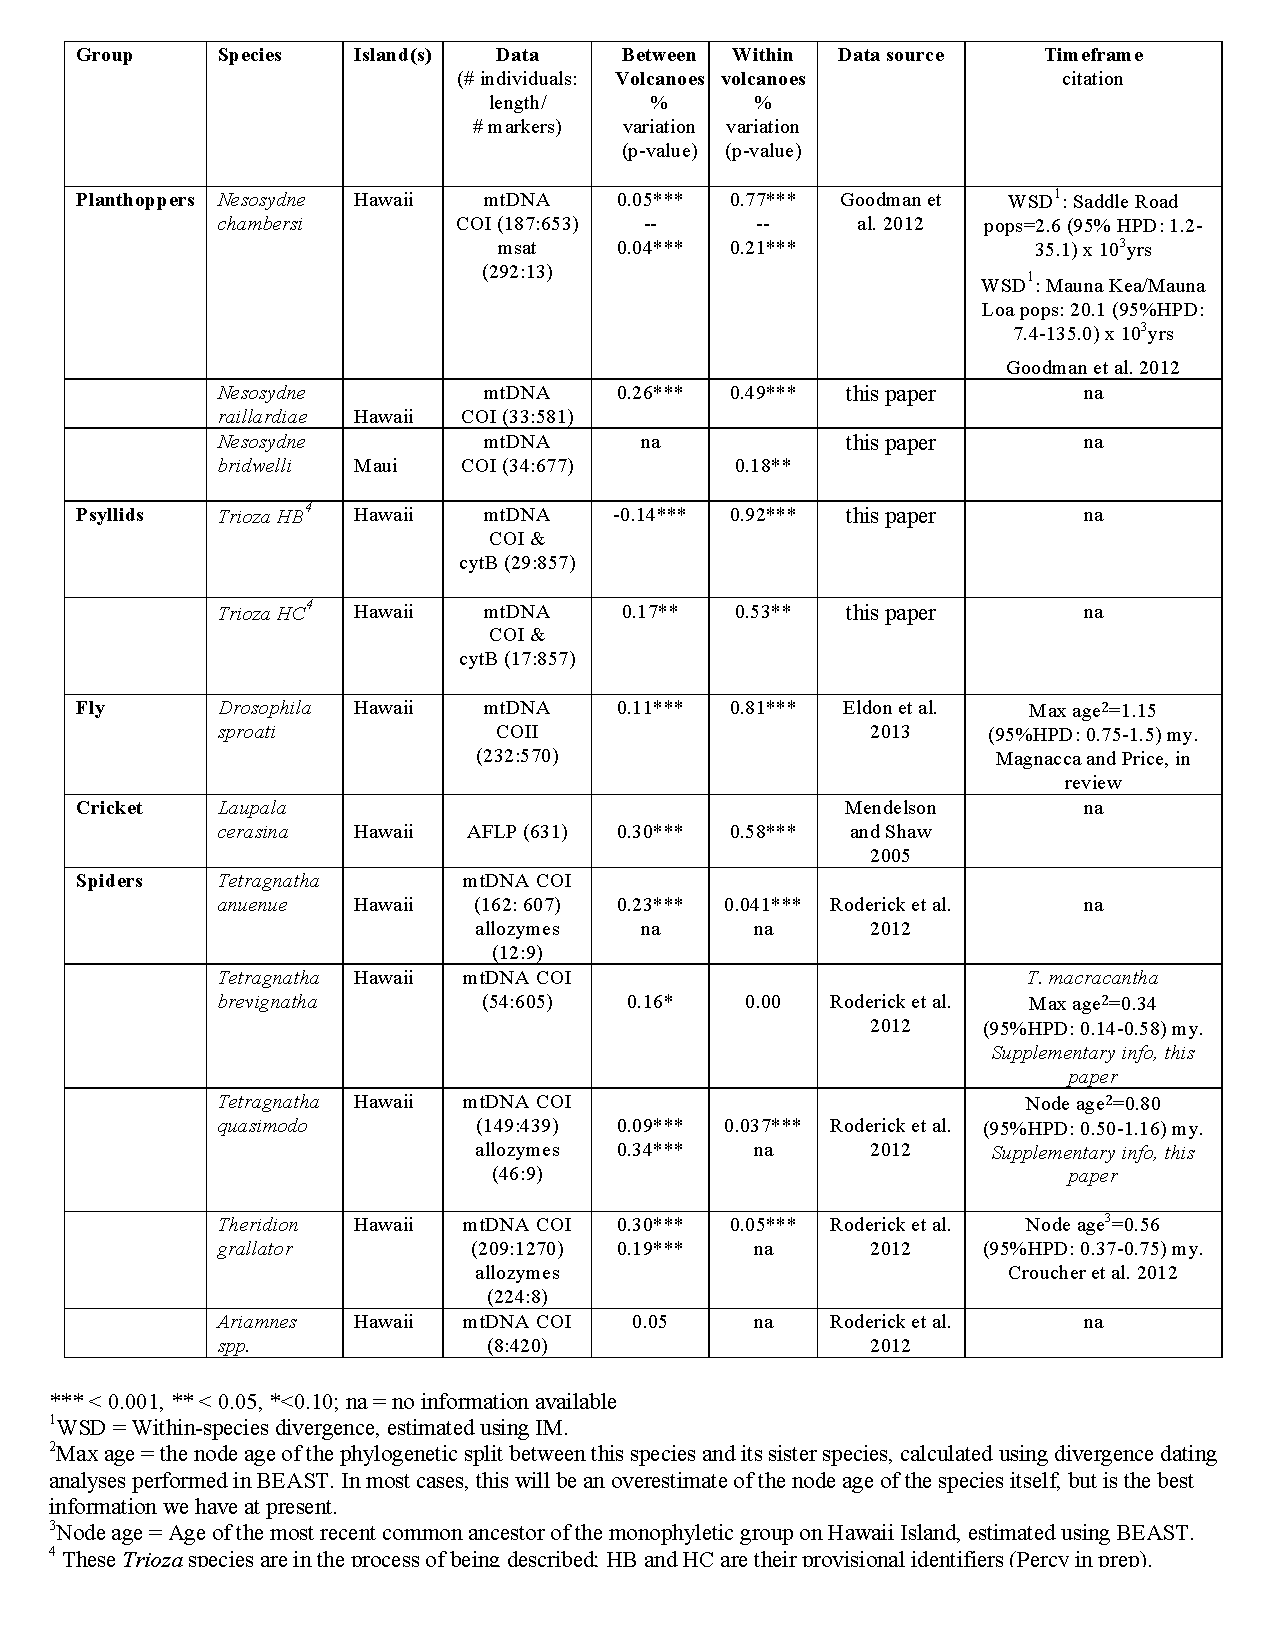
\includegraphics[width=0.9\textwidth]{../tab_fst.pdf}
  \caption{Proportion of genetic variation distributed at between
    volcanoes and among sites within volcanoes.}
  \label{tab:fst}
\end{table}

\clearpage

\section*{Figure captions}


{\bf Figure 1.} Substrate age map of the islands of Kauai, Maui and
Hawaii Island. Colors correspond to substrate age from young (yellow)
to old (blue). Focal sites are shown as black circles while sampling
sites for genetic data are represented by gray circles.

\vspace{2em}
\noindent {\bf Figure 2.} Genetic population structure ($F_{ST}$)
among sites within volcanoes with volcano age for insects and
spiders. The plant-feeding groups, specifically the sap-feeding
Hemiptera, show high genetic structure among sites on young volcanoes
relative to older volcanoes whereas detritivores (crickets),
fungivores ({\it Drosophila}), and in particular predators (spiders),
show little structure on young volcanoes. For spiders, substantial
structure develops only later in the chronosequence, e.g., on Maui at
approximately 1 million years. Number refer to different species:
1. {\it Nesosydne chambersi}, 2. {\it Nesosydne raillardiae}, 3. {\it
  Nesosydne bridwelli}, 4. {\it Trioza HB}, 5. {\it Trioza HC},
6. {\it Drosophila sproati}, 7. {\it Laupala cerasina}, 8. {\it
  Tetragnatha anuenue}, 9. {\it Tetragnatha brevignatha}, 10. {\it
  Tetragnatha quasimodo}, 11. {\it Theridion grallator}.

\vspace{2em}
\noindent
{\bf Figure 3.} Patterns in degree distributions across sites and
different biogeographic classifications of taxa. Top panels show that
networks deviate most from MaxEnt on youngest and oldest sites. Inset
figures show the distribution of simulated mean squared errors; if the
red line falls within the gray region (95\% confidence interval) the
data conform to maximum entropy; thus the observed minor deviation on
Kohala is not different than expected by chance. Kohala shows minimal
modularity, and maximal connectance. The bottom panel shows the number
of links for island endemics versus island cosmopolitans. Endemics
show lower linkage overall, but significantly increase on the middle
aged site Maui (highlighted with dotted box). Kohala shows increased
linkage overall (highlighted with solid box). When looking at links to
plant genera this pattern holds except that endemics on Maui no long
show a difference in generality, indicating that the pattern is driven
in part by plant diversity.

\vspace{2em}
\noindent
{\bf Figure 4.} Trends in network metric nestedness and modularity
through time. Nestedness decreases while modularity increases. Error
bars come from a null model simulation. While the sign of the z-score
depends on null model and method of calculating modules (see
supplemental figure) the overall trend is robust. Some level of
nestedness is likely a statistical property of these networks, however
it could also be driven by stabilizing ecological
mechanisms. Modularity is thought to be a sign of coevolution driving
convergence in traits of plants and herbivores. Note the very
interesting peaks on Maui where adaptive diversification may be at its
maximum.

\clearpage

\section*{Figures}

\begin{figure}[!htb]
  \centering
  \includegraphics[scale=0.7]{../fig_map.pdf} 
  \caption{}
  \label{fig:map}
\end{figure}

\begin{figure}[!hp]
  \centering
  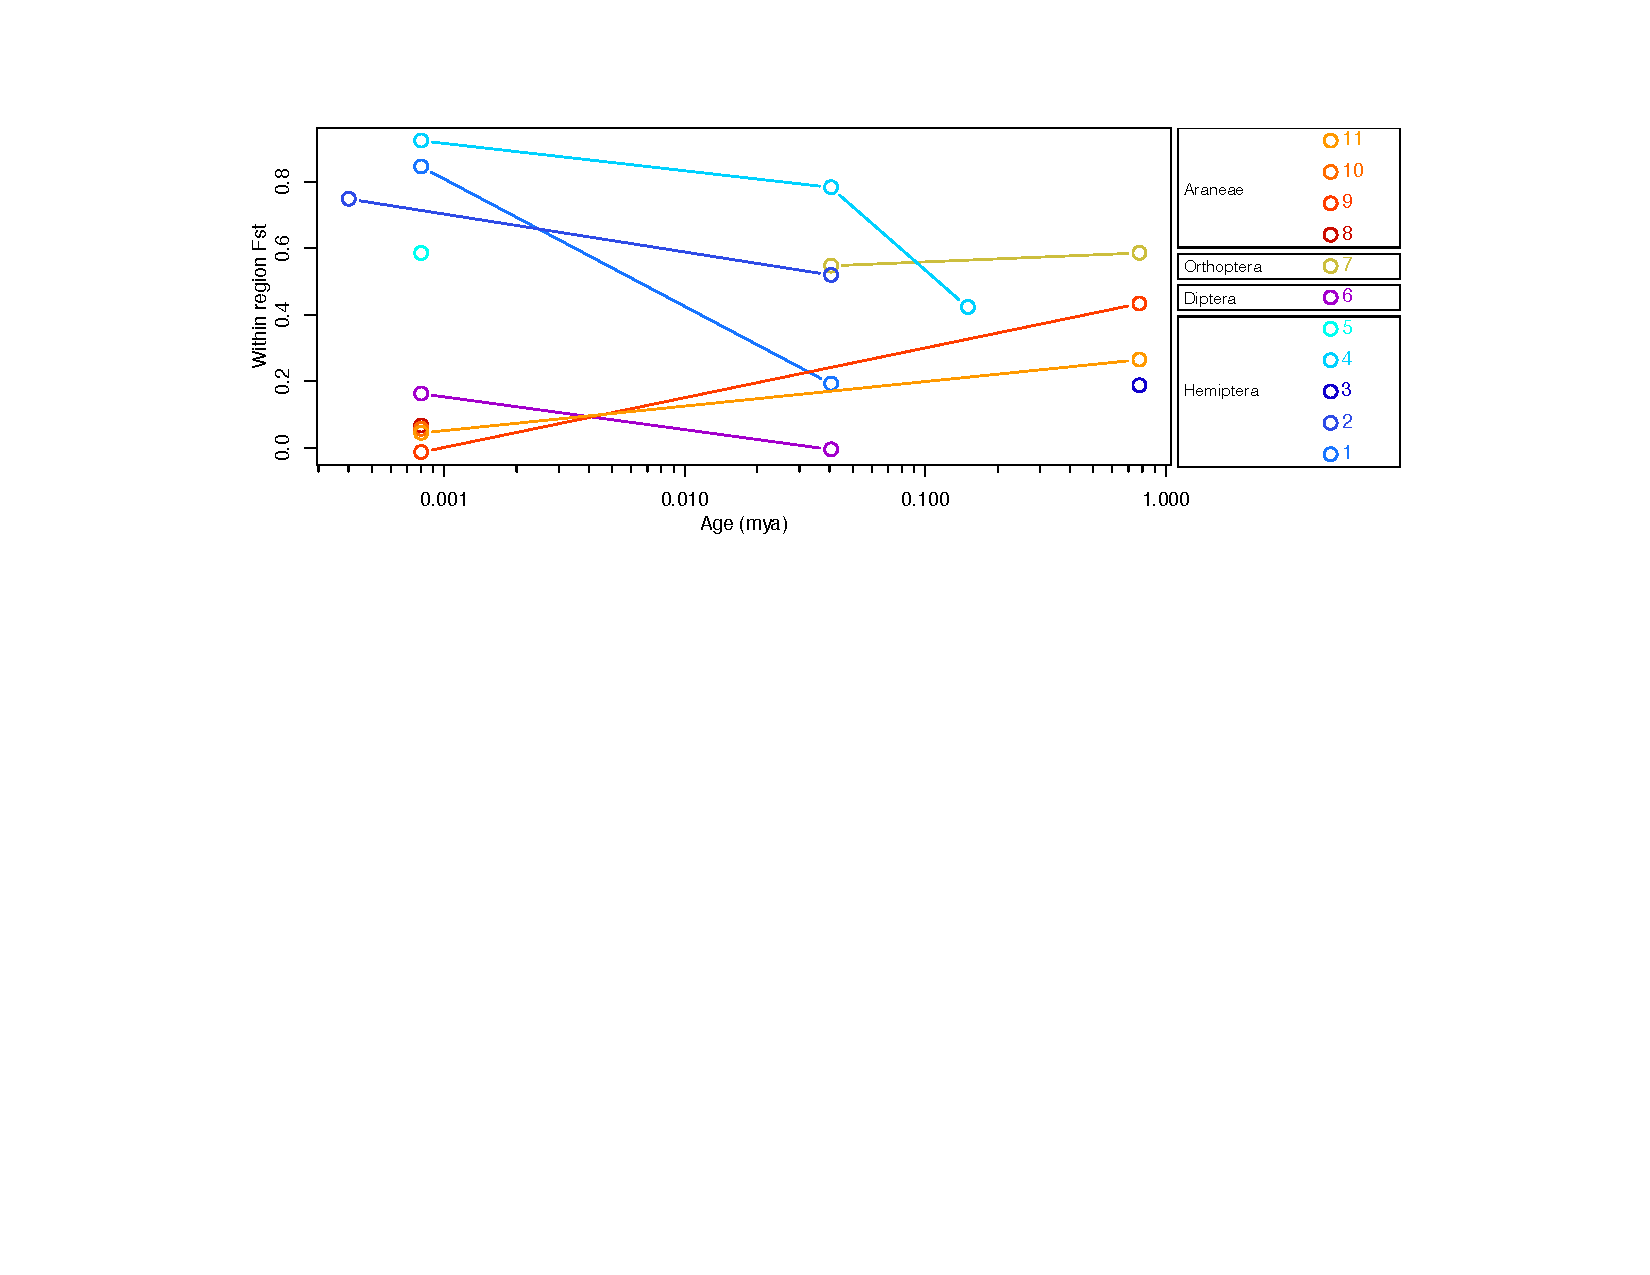
\includegraphics[scale=0.7]{../fig_volcanoFst.pdf}
  \caption{}
  \label{fig:volcanoFst}
\end{figure}

\begin{figure}[!hp]
  \centering
  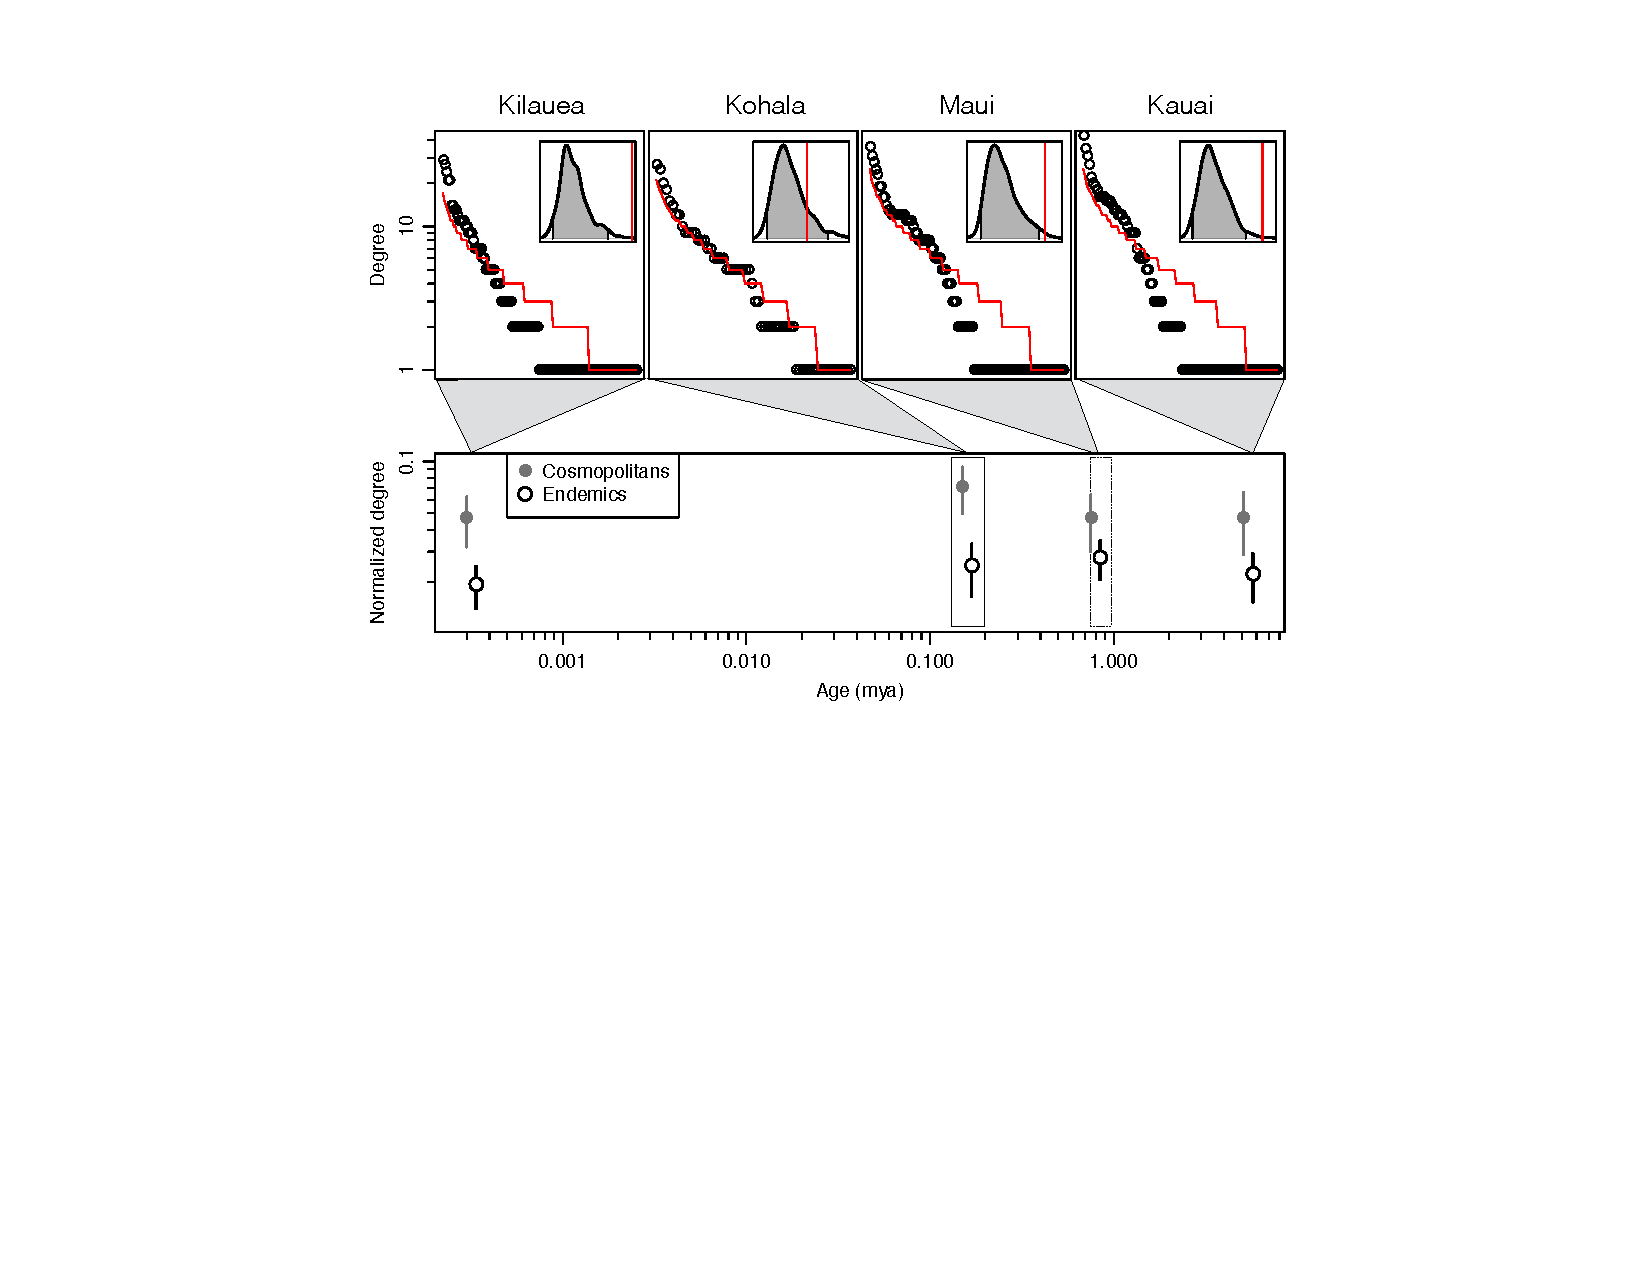
\includegraphics[scale=0.8]{../fig_degree.pdf} 
  \caption{}
  \label{fig:degree}
\end{figure}

\begin{figure}[!hp]
  \centering
  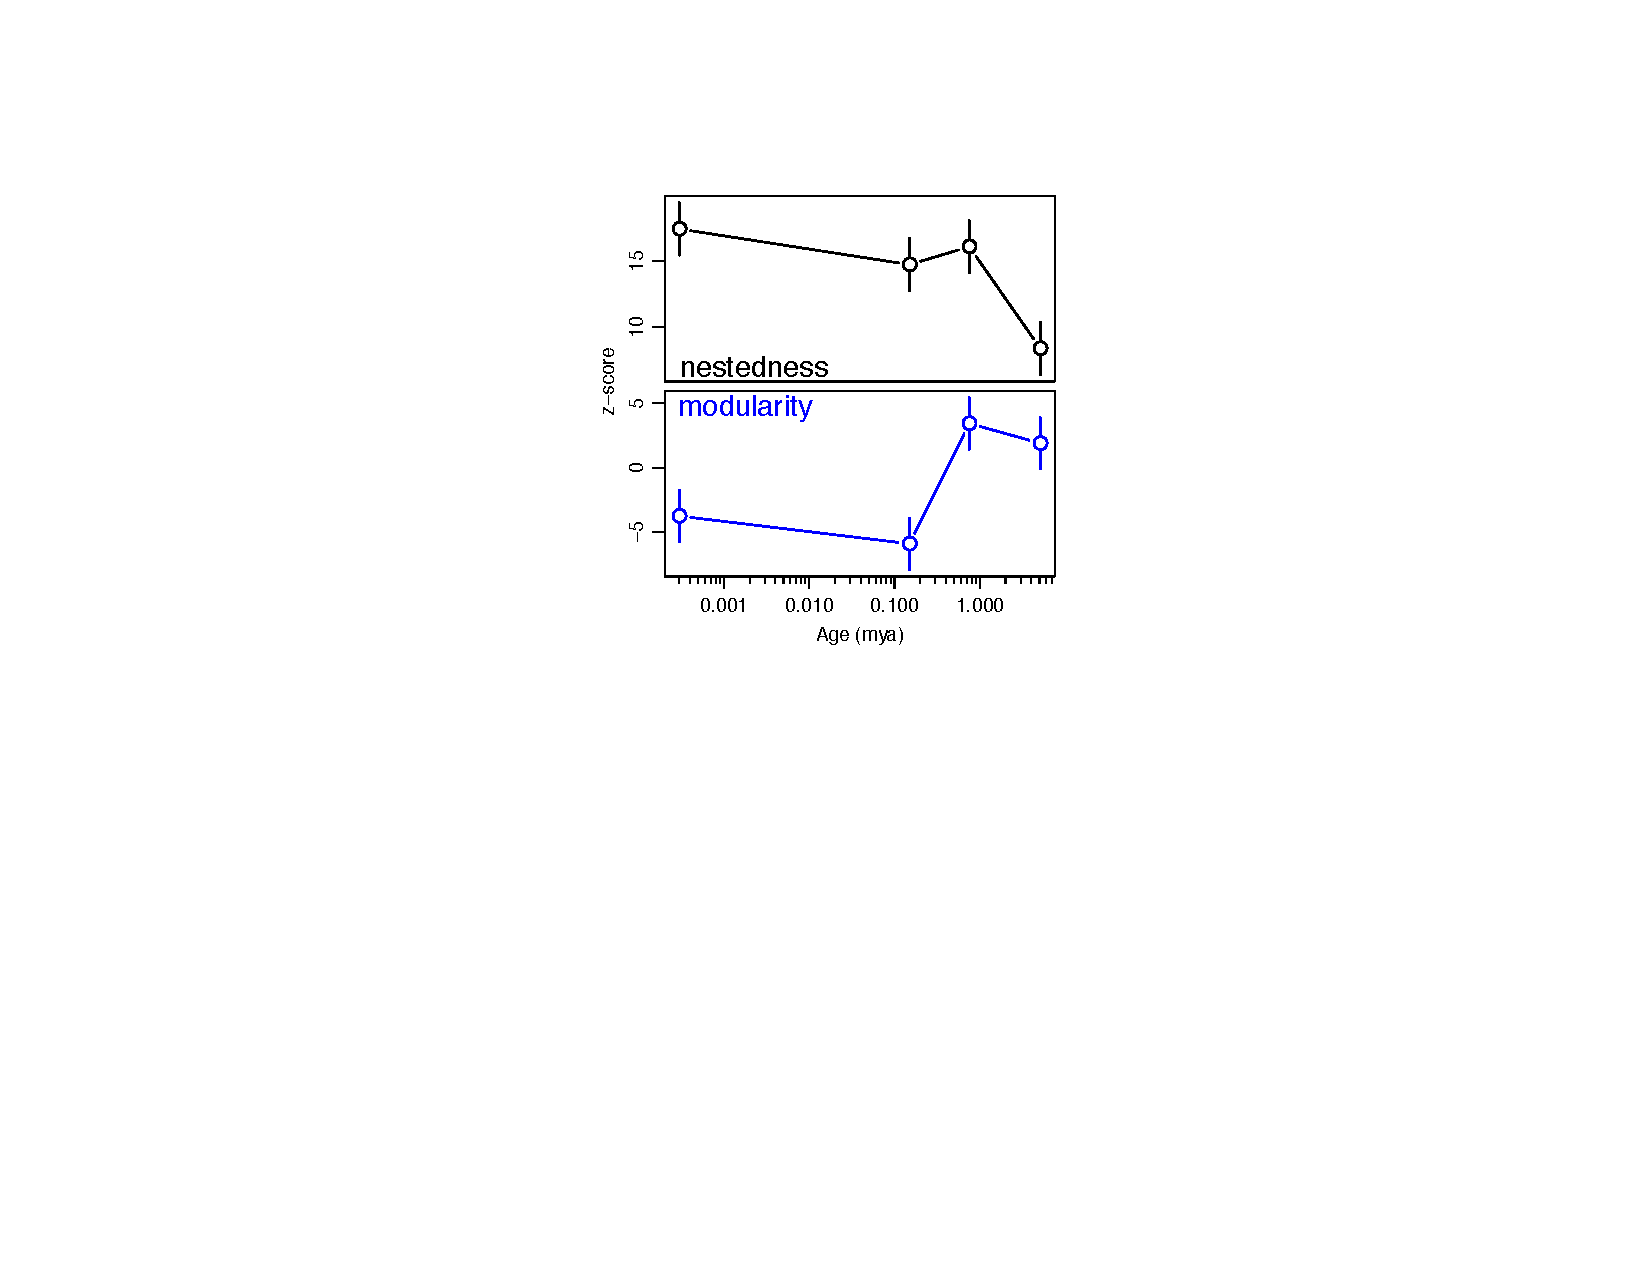
\includegraphics[scale=1]{../fig_netMets.pdf} 
  \caption{}
  \label{fig:netMet}
\end{figure}

\end{linenumbers}

\end{document}

